\documentclass{article} % For LaTeX2e
\usepackage{nips15submit_e,times}
\usepackage{hyperref}
\usepackage{url}
\usepackage{graphicx}
%\documentstyle[nips14submit_09,times,art10]{article} % For LaTeX 2.09


\title{Face Emotion Classification Using Single-Layer Neural Networks}


\author{
Kexiang Feng \\
Department of Computer Science and Engineering\\
University of California, San Diego\\
\texttt{fkxcole@gmail.com} \\
\And
Xupeng Yu \\
Department of Electrical and Computer Engineering \\
University of California, San Diego \\
\texttt{xuy004@eng.ucsd.edu}
}

% The \author macro works with any number of authors. There are two commands
% used to separate the names and addresses of multiple authors: \And and \AND.
%
% Using \And between authors leaves it to \LaTeX{} to determine where to break
% the lines. Using \AND forces a linebreak at that point. So, if \LaTeX{}
% puts 3 of 4 authors names on the first line, and the last on the second
% line, try using \AND instead of \And before the third author name.

\newcommand{\fix}{\marginpar{FIX}}
\newcommand{\new}{\marginpar{NEW}}

\nipsfinalcopy % Uncomment for camera-ready version

\begin{document}


\maketitle

\begin{abstract}
Nowadays, there are many machine learning libraries to help us simplify the process of building a machine learning system like a facial emotion recognition neural network. In this paper, we manage to implement a facial emotion recognition system without using any of these libraries. We start with a logistic regression layer to solve the binary classification problem, then we extend our effort to more general multi-label classifications with the help of the softmax layer. We also use Principal Components Analysis to simplify the calculation. Our models are evaluated on the CK+ dataset using 10-fold cross-validation. Our logistic regressor achieves an average accuracy of $ 100\% $ in Happy vs Angry classification and our softmax regressor achieves an average accuracy of 78\% in 6-way classification. We hope our efforts can clearly explain the composition of a complete machine learning system. 
\end{abstract}

\section{Introduction}
A powerful tool in the machine learning area is the various libraries like Sklearn and Pytorch. One primary problem of using built-in functions is that it makes people unwilling to understand how they actually work. However, it is quite important to analyze the math expressions if we want to improve the whole system. We, therefore, investigate the whole process by implementing Logistic regression and the relating knowledge ourselves. The key value of our work is to help summarize the Logistic Regression with a simple emotion recognition example.

\section{Method}
Our discussion is made up of 5 sections. In section 1, we briefly introduce our data preprocessing and data split, namely Principal Component Analysis and K-Fold. Section 2 and 3 elaborate our work in the logistic regressor and softmax regressor. Following that we share our findings in Section 4. Lastly, we briefly introduce individual contributions in section 5.

\section{Dataset and Task Description}
In this problem, we use facial expressions from the Extended Cohn-Kanade Dataset(CK+). CK+ is a widely used dataset for action unit
and emotion-specified expression. It extends CK released in 2000 by including more subjects and sequences. We use six classes of aligned emotions each of which includes different numbers of 192*224 pictures and two classes of resized emotions each of which includes different numbers of 160*122 pictures. Resized images include the background therefore the percentage of the face is smaller while the aligned images cut off the background and make the face fulfill the images. 
Our task includes two parts: One is the comparison of performance on resized and aligned images and the other is the multiclass classification problem. We will preprocess the images in three ways: performing PCA, choosing balanced data and using K-Fold Cross Validation which will be described below.
\begin{figure}	
	\centering
	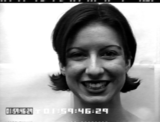
\includegraphics[scale=1]{./graph/resized_sample.png}
	\caption{A sample from the resized images}
\end{figure}
\begin{figure}	
	\centering
	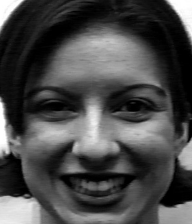
\includegraphics[scale=0.6]{./graph/aligned_sample.png}
	\caption{A sample from the aligned images}
\end{figure}
\subsection {Data Balance}
In this problem, we mainly use a balanced dataset, which means we use the same amount of each image in each class. Balancing is completed by choosing the first $n$ images, where $n$ is the least number of images in each class. For most of our problems, we will use a balanced dataset, and we try to look further into the imbalanced dataset problem in the last part of our work.
\subsection {Principal Component Analysis}
PCA, namely Principal Component Analysis, in high dimensional data analysis, especially in the field of image processing. For example, if we have a 100*100 pixel image, it is usually computational expensive to throw all the information into the network. Therefore, PCA simplifies the calculation by choosing the eigenvector with the largest k singular values, which are intuitively the main feature of the image. However, the traditional way of PCA preforming has the following problem: if a picture has 100*100 pixels, we have to compute the covariance matrix of 100*100 elements. To avoid such a hard task, we introduce the Turk \& Pentland’s Trick. IF there are M pictures of N*N size, we first form a  $N^2 \times M$ matrix and substrate the mean of the pixels, then we get a matrix M.
Then instead of calculating the covariance of A which is $AA^T$, we use $A^TA$.This is because we find the relationship between the eigenvectors of the two matrices.
$$A^{T} A v_{k}=\lambda_{k} v_{k}$$
$$A A^{T} A v_{k}=A \lambda_{k} v_{k}=\lambda_{k} A v_{k}$$
$$A A^{T} \hat{u}_{k}=\lambda_{k} \hat{u}_{k}$$
So the eigenvector for $A A^{T}$ is $u_{k}=\frac{\hat{u}_{k}}{\left\|\hat{u}_{k}\right\|}$.\\
And our method passes the sanity check which proves it to be a reasonable way.
Result: We choose different numbers of components of the PCA result and test their performance in two-classes and six-classes problems. The result is shown below.
\begin{table}[!htbp]
\centering
\begin{tabular}{ccc}
\hline
n components&avg accuracy& avg loss\\
\hline
3& 0.605& 0.674753\\
5& 0.9775& 0.546476\\
8&0.99&0.533554\\
10&0.98& 0.532621\\
\hline
\end{tabular}
\caption{PCA performance under binary classification problem}
\end{table}
\begin{table}[!htbp]
	\centering
	\begin{tabular}{ccc}
		\hline
		n components&avg accuracy& avg loss\\
		\hline
		10& 0.527778& 1.201420\\
		20& 0.697222& 0.921799\\
		40& 0.788889& 0.757366\\
		50& 0.780556& 0.726486\\
		\hline
	\end{tabular}
	\caption{PCA performance under six class classification problem}
\end{table}
\subsection {K-Fold Cross Validation}
To make full use of the data to estimate our model’s average performance, we introduce k-fold cross-validation, where we let k equals 10 here. We divide the dataset into 10 folds. For each time, we choose one fold to be valid data, one fold to be test data and the rest to be train data. After running ten times, we calculate the average train loss, valid loss and test loss. To make sure a balanced dataset, for each fold we choose the same number of pictures in each class. Our experiments result below are all based on the K-Fold Cross Validation process. 

\section{LOGISTIC REGRESSION}
Logistic regression is a basic idea used in the binary classification field. It is developed from the linear regression model and it can also be modified to softmax regression model to do multiclass classification, which we will discuss below. There are two main parts in the process. \\
One part is to calculate the loss and prediction of valid data according to the model parameters. Different from linear regression, we use the sigmoid function at the output to make it in $[0,1]$. 
$$h_{\theta}(x)=g\left(\theta^{T} x\right)$$
$$g(z)=\frac{1}{1+e^{-z}}$$
$$ J(\theta) = =-\frac{1}{m}\left[\sum_{i=1}^{m} y^{(i)} \log h_{\theta}\left(x^{(i)}\right)+\left(1-y^{(i)}\right) \log \left(1-h_{\theta}\left(x^{(i)}\right)\right)\right]$$
And then we use the loss and prediction to calculate parameters and modify the model parameters. The process is called gradient descent.
$$\theta_{j}:=\theta_{j}-\alpha \frac{\partial}{\partial \theta_{j}} J(\theta)$$
$$\theta_{j}:=\theta_{j}-\alpha \sum_{i=1}^{m}\left(h_{\theta}\left(x^{(i)}\right)-y^{(i)}\right) x_{j}^{(i)}$$
There are two kinds of gradient descent, batch gradient descent and stochastic gradient descent. The former one update the parameters once every epoch and the latter one update the parameters after every data in an epoch.\\
With a good learning rate $\alpha$, we can see valid loss going down. We then test Logistic Regression on different datasets shown below.
\subsection {Evaluation on Happiness vs Anger using the resized dataset}
Here we perform logistic regression on the happy and angry faces from the resized dataset once. The training loss and validation loss are shown below.
From Figure3, we can see that with the increase of epoch, the training loss continuously goes down while the validation loss goes down and then up again. And the test accuracy is 0.37500.
\begin{figure}[htb]
	\centering
	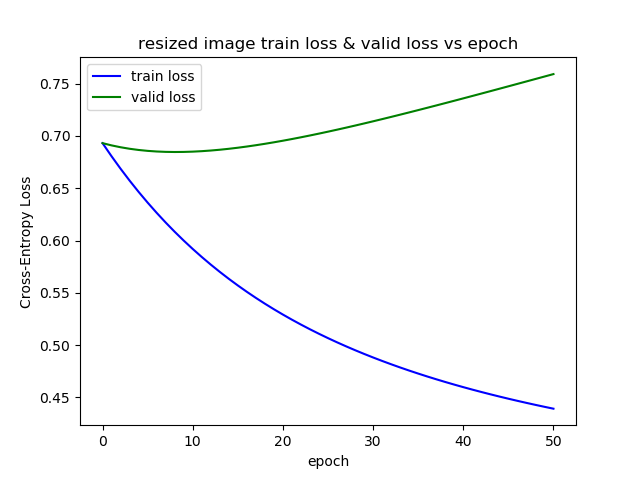
\includegraphics[scale=0.5]{./graph/resized_tvloss.png}
	\caption{resized image train loss \& valid loss vs epoch(happiness and anger)}
\end{figure} 
This is quite a bad result of overfit. \\
Therefore, Figure 4 plots the first four principal components of the resized data. As shown, the most important 4 principal components do not give any information about facial emotion. Therefore, we want to perform our data on the aligned dataset.
\begin{figure}[h]
	\centering
	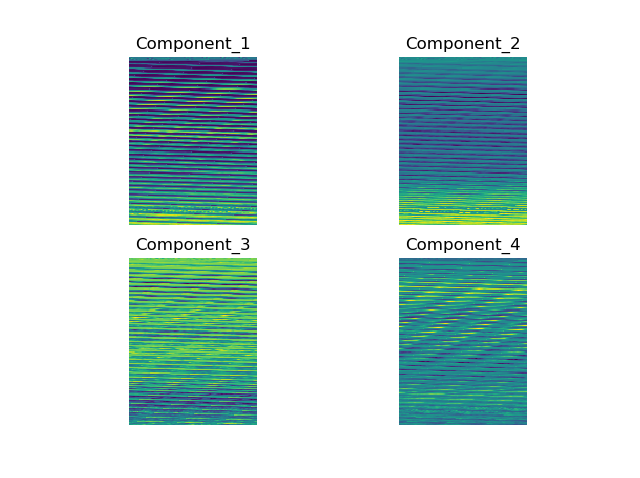
\includegraphics[scale=0.5]{./graph/pca_resized.png}
	\caption{First four principal components of the resized data}
\end{figure} 
\subsection {Evaluation on Happiness vs Anger using the aligned dataset}
Again in this problem, we test the Logistic Regression on aligned dataset.
\begin{figure}[h]
	\centering
	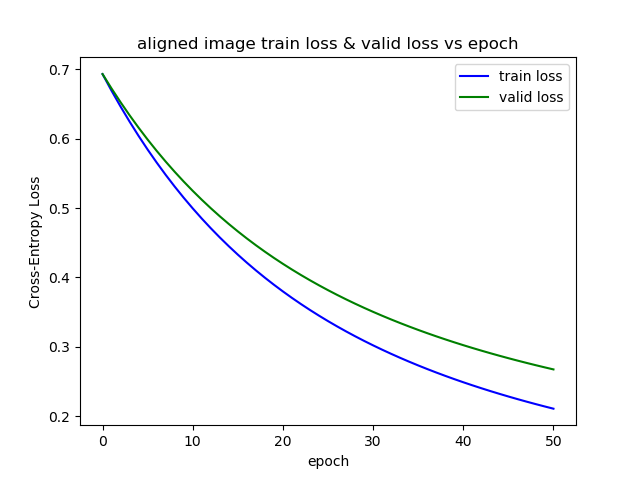
\includegraphics[scale=0.5]{./graph/aligned_tvloss.png}
	\caption{aligned image train loss \& valid loss vs epoch(happiness and anger)}
\end{figure}
As Figure5 shows, this time the validation loss goes down with training loss. And the test accuracy reaches 1.0. Figure 6 shows the first four principal components of the aligned data. This time the principal components become quite meaningful. This is the reason for the outstanding performance.
\begin{figure}[h]
	\centering
	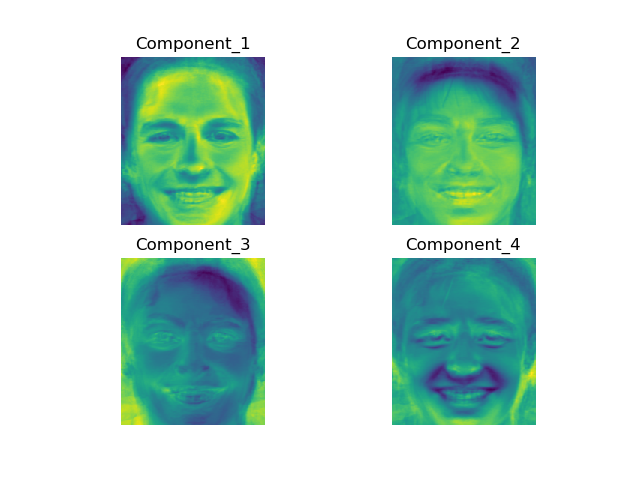
\includegraphics[scale=0.5]{./graph/pca_aligned.png}
	\caption{First four principal components of the aligned data}
\end{figure}
When we choose learning rate = 0.1 and 50 components, the test accuracy reaches 1.0. That means we successfully classified all the data!\\
\begin{figure}[h]
	\centering
	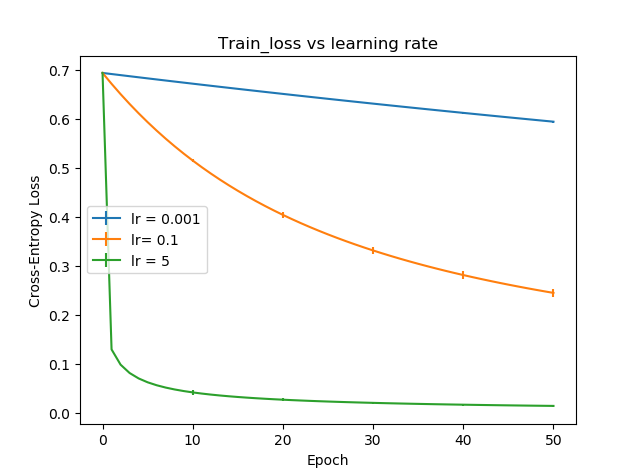
\includegraphics[scale=0.5]{./graph/diff_lr.png}
	\caption{The influence of three different learning rates on train loss(happiness and anger)}
\end{figure}
We use 50 components to test the influence of learning rate on train loss. As Figure 7 shows, when the learning rate is too high, we cannot track the trend smoothly and the test accuracy is the lowest under learning rate 0.1, so 0.1 is a reasonable learning rate for this problem.
\subsection {Evaluation on Fear vs Surprise using the aligned dataset}
Figure 8 shows the training loss and valid loss on Fear vs Surprise using the aligned dataset. The valid loss still goes down with train loss. And the accuracy reaches 0.958. Therefore, happiness vs anger is not a special case. The aligned dataset does outstand the resized dataset. This is because aligned data centers the face and throws the useless background information away. So the principal components can more focus on the emotion difference.
\begin{figure}[h]
	\centering
	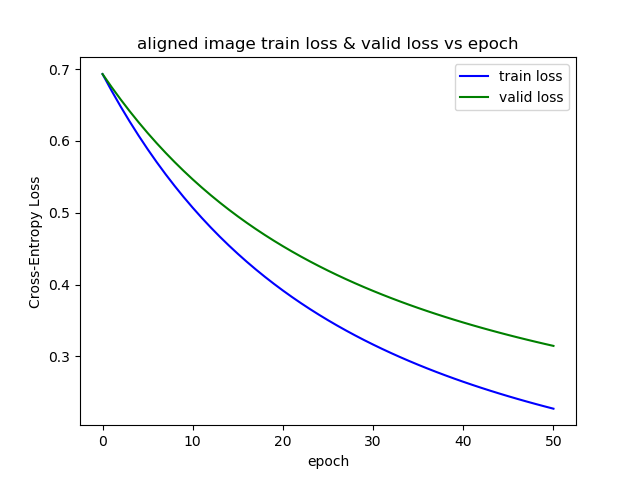
\includegraphics[scale=0.5]{./graph/aligned_angerfear.png}
	\caption{aligned image train loss \& valid loss vs epoch(surprise and fear)}
\end{figure}

\section{SOFTMAX REGRESSION}
Softmax is the generalization of logistic regression for multiple classes. Given an input $x^n$, softmax regression will output a vector $y^n$, where each element, $y_k^n$ represents the probability that $x^n$ is in class k.
\subsection {Model Evaluation}
We performed an 10-fold cross validation on pictures of six emotions to check our model's performance. In each fold, best model parameters is selected so that holdout dataset reaches lowest loss. Then we use the model parameters to record the accuracy on test dataset. Final model performance is the average recorded accuracy of ten folds. \\
Figure9 shows the training process and Figure10 shows the result in confusion matrix form.
\begin{figure}[h]
	\centering
	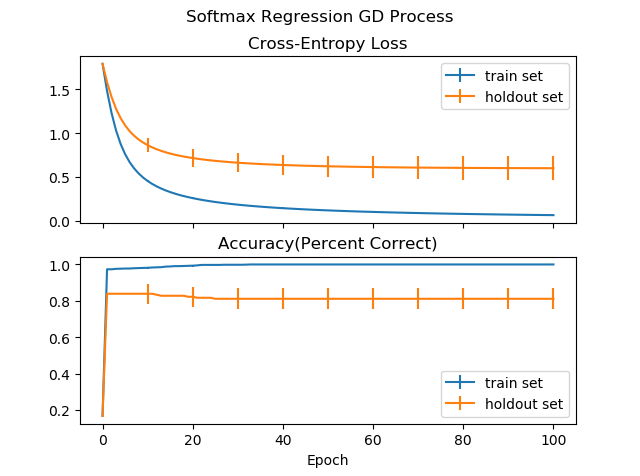
\includegraphics[scale=0.5]{./graph/softmax_tvloss_acc.png}
	\caption{train \& valid loss-accuracy vs epoch(six emotions)}
\end{figure}
\begin{figure}[h]
	\centering
	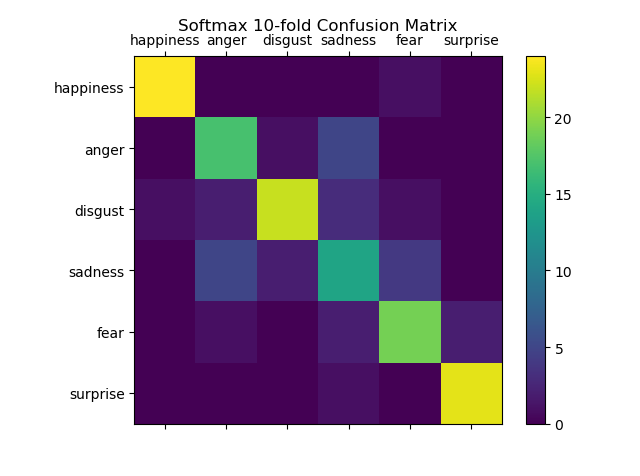
\includegraphics[scale=0.5]{./graph/confusion.png}
	\caption{Softmax 10-fold Confusion Matrix}
\end{figure} 
\subsection {Batch vs Stochastic Gradient Descent}
In normal batch gradien descent(GD), weights are updated once per epoch. To increase the converging speed over every epoch, stochastic gradient descent(SGD) is introduced.\\
The figure below compares the converging speed between GD and SGD. We can see that SGD is much faster in terms of minimizing the loss in fewer epochs. The reason is that in each SGD epoch, model parameters are updated N times(N is the training set size) instead of one time.
\begin{figure}[h]
	\centering
	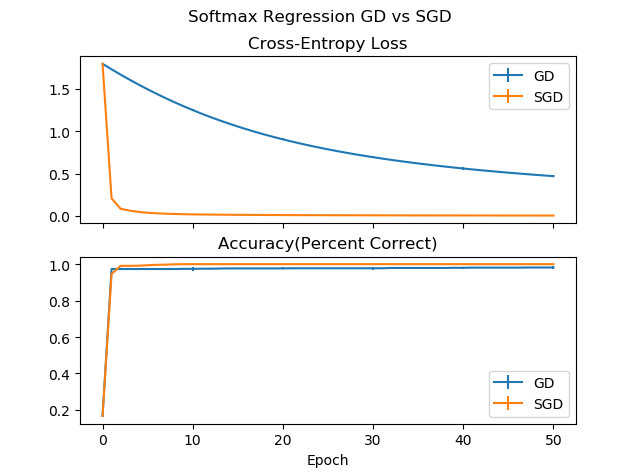
\includegraphics[scale=0.5]{./graph/gd_vs_sgd.png}
	\caption{Softmax 10-fold Confusion Matrix}
\end{figure}
\subsection {Weight Visualization}
To show that our model has learned meaningful patterns, we can visualize the model parameters by doing inner product with our PCA components. Below pictures show the result of visualized weights.
\begin{figure}[h]
	\centering
	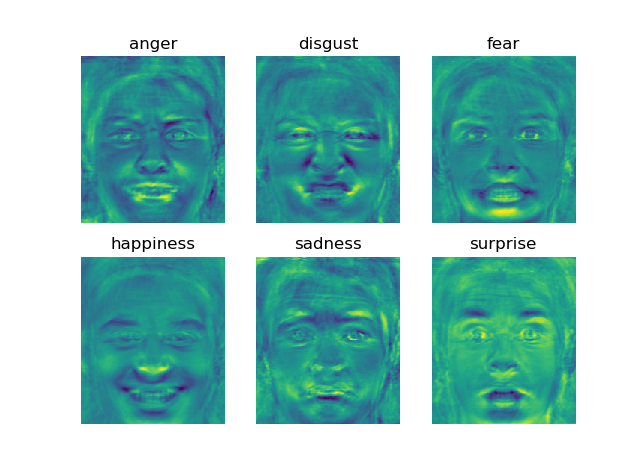
\includegraphics[scale=0.5]{./graph/softmax_weight.png}
	\caption{Softmax 10-fold Confusion Matrix}
\end{figure}
\subsection {Class weights to handle imbalanced dataset}
The above experiments have been performed on a balanced dataset. In order to handle imbalanced dataset, we modify our model by adding class weights. The basic idea is that we want to give a penalty to the major classes and a bonus to the rare classes. Class weights are defined as $c_k = C*N/N_k$ where C is class number, N is sample number and $N_k$ is sample number with class k. \\
Given this class weight definition, we define weighted cross entropy $E = -\sum_{n}\sum_{k=1}^{C} c_k t_k^n ln y_k^n $ as our loss function. The target of our new model training process is to minimize the weighted cross entropy. \\
Below figure compares the modified model with the original model using the whole CK+ dataset.
\begin{figure}[h]
	\centering
	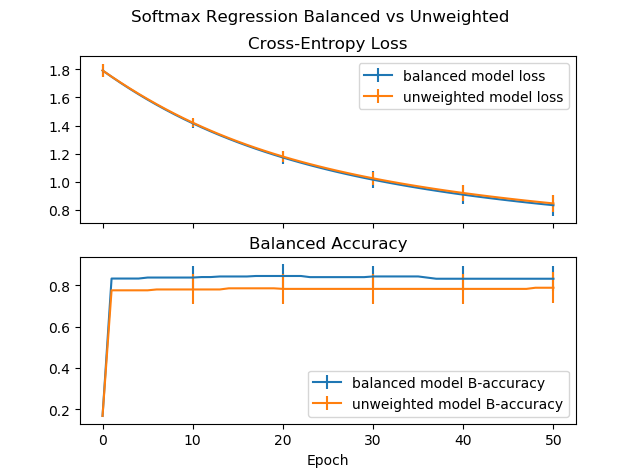
\includegraphics[scale=0.5]{./graph/unbalanced.png}
	\caption{Softmax Regression Balanced vs Unweighted}
\end{figure}
\section {CONCLUSION}
From the discussion above, the power of Logistic Regression and Softmax Regression not only depends on the algorithm itself but also relies on the data and preprocessing.
A nice dataset is always helpful. To solve the problem of an unbalanced dataset, we should choose some amount of data from each class or add weight to data. To avoid calculating high dimension data, we can use PCA and the Turk \& Pentland's trick. An ideal image in the dataset should get rid of the background and focus on the region of consideration.\\
Other tricks are also helpful. For example, K-fold Cross-Validation can help us make full use of the dataset and choose a good model.\\
For the algorithm itself, we should focus on the learning rate and early stopping problem. A good learning rate can speed up gradient descent as well as track the trend well. For this problem, the learning rate should be about 0.1. In the resized dataset, we can see the valid loss does not go down as train loss due to overfitting. Therefore we should also care about the intermediate process and use early stopping to record the best parameters.
\section{INDIVIDUAL CONTRIBUTIONS}
Our group consists of two members: \textit{Kexiang Feng} and \textit{Xupeng Yu}. \\
\textit{Kexiang Feng} builds the PCA, K-Fold modules and Softmax regressor. He also wrote the scripts to visualize the softmax weights and PCA components. \\
\textit{Xupeng Yu} built the Logistic regressor and finished the relating binary classification problem. He also collected the figures and wrote the main report. 


\bibliographystyle{plain}
\bibliography{ref}
\end{document}
